\documentclass[a4paper,11pt]{article}
\usepackage[T1]{fontenc}
\usepackage[italian,english]{babel}
\usepackage[utf8]{inputenc}

\usepackage[hidelinks, colorlinks=false]{hyperref}
\usepackage{graphicx}
\usepackage{bookmark}

\makeindex


\begin{document}



\title{SWE-B: Leggere tra le righe}
\author{Eduard Bicego}
\date{23-05-2016}

\maketitle

\tableofcontents
\newpage
\listoffigures
\newpage


\section{Diagrammi delle classi}

	\subsection{Iterator Pattern}
	
	\begin{quote}
		\textit{"sequenza di amminoacidi"}
	\end{quote}
	
	Attenzione, quando si descrive una collezione, sequenza e insieme è richiesto l'inserimento dell'\textbf{ITERATOR}. Evita la tentazione di usare Collection Java, l'implementazione del pattern è uguale e ti farà guadagnare più punti.
			
			\begin{figure} [h]
				\centering
				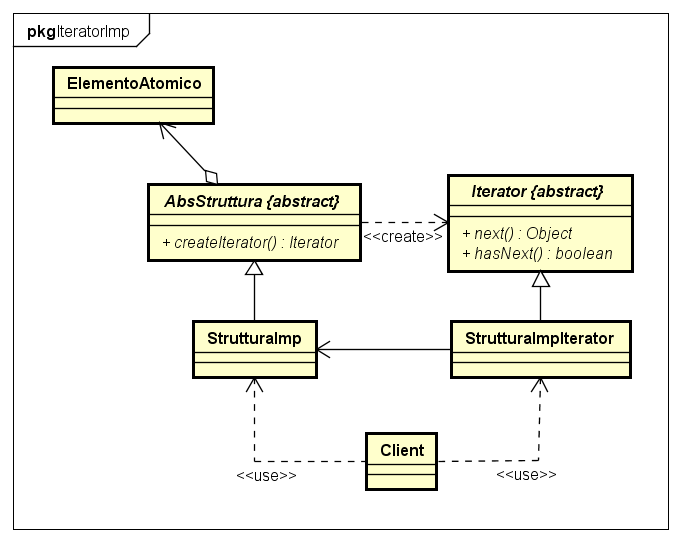
\includegraphics[scale=0.5]{ClassDiagramPattern/IteratorImp/IteratorImp}
				\caption{Iterator}
				\label{fig:IteratorImp}
			\end{figure}


\newpage
	\subsection{Strategy e Template Pattern}
	
	\begin{quote}
		\textit{"Il sistema, successivamente, utilizza un algoritmo di ricerca su database esterni per individuare la proteina codificata dagli amminoacidi."}
	\end{quote}
	
	In generale quando c'è la parola \textbf{ALGORITMO} o c'è da utilizzare lo \textbf{STRATEGY} o il \textbf{TEMPLATE}.
	
	\begin{quote}
		\textit{"Nella versione attuale del software l'algoritmo è ancora poco efficiente ed  utilizza una ricerca lineare sulla lista degli amminoacidi, iterando su di essa in modo  sequenziale. Poiché gli sviluppatori hanno in progetto di rendere più efficiente tale  processo, hanno modellato il sistema in modo tale da poterlo facilmente estendere con nuovi algoritmi."}
	\end{quote}
	
	Quando si parla di \textit{ALGORITMO} ed è specificato che tale \textit{ALGORITMO} verrà esteso con \textit{NUOVI ALGORITMI} e reso più efficiente si parla di \textbf{STRATEGY}. Anche il \textbf{TEMPLATE} avrebbe senso ma lo \textbf{STRATEGY} è più semplice ed accettato.
	
	\begin{quote}
		\textit{"È possibile scegliere fra tre tipologie di giocatori guidati dal computer, ad ognuno dei quali corrisponde un modello di intelligenza artificiale via via migliore."}
	\end{quote}
	
	Intelligenza artificiale, algoritmi che cambiando sono via via migliori. Sempre usare lo \textbf{STRATEGY} in questi casi. "guidati dal computer" in questo caso esplicita chi ha la relazione con la gerarchia.
	
	\begin{quote}
		\textit{"Sulla base del formato del libro, che può essere AZW3, PDF, MOBI, il sistema operativo seleziona un algoritmo differente di resa a video (impaginazione) che determina la prossima pagina da leggere."}
	\end{quote}
	
	Altro caso, quando si parla di 'formati' e si elenca una lista abbiamo ancora lo \textbf{STRATEGY}. In questo caso si specifica anche chi utilizza l'astrazione della gerarchia dello \textbf{STRATEGY}, ossia il sistema (il \textbf{Controller}).
	
	\begin{quote}
		\textit{"Le richieste HTTP possono essere codificate sia in XML sia in JSON"}
	\end{quote}
	Necessario utilizzare un pattern \textbf{STRATEGY}, in questo caso per il Parser (codificazione) dei due formati.
	
	Spesso la relazione con la superclasse della gerarchia dello \textbf{STRATEGY} e scritta nel testo.
	
			\begin{figure} [h]
					\centering
					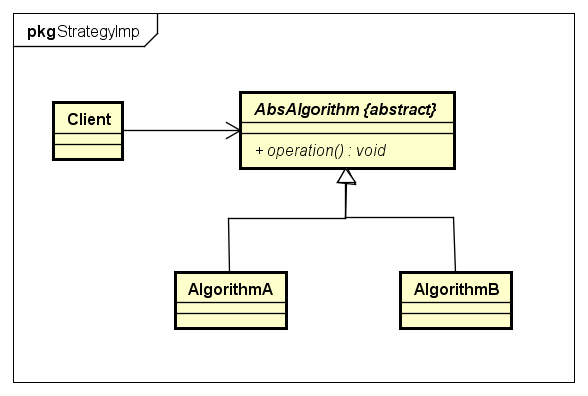
\includegraphics[scale=0.6]{classDiagramPattern/StrategyImp/StrategyImp}
					\caption{Strategy + client}
					\label{fig:StrategyImp}
			\end{figure}
	
	\begin{quote}
		\textit{"La componente che visualizza le immagini sullo schermo, applica una funzione di rendering che differisce solo in parte sulla base del formato, ma che possiede numerose parti in comune fra le immagini in MP4 e in MVK"}
	\end{quote}
	
	Quando c'è la terminologia \textit{'in parte'} o \textit{'parti'} si riferisce chiaramente all'uso di un \textbf{TEMPLATE}. 
	
	\begin{quote}
		\textit{"La trasformazione degli oggetti in istruzioni per le testine avviene utilizzando un apposito componente. Parte delle istruzioni sono comuni per entrambi i tipi di dato, parte è invece dipendente dal tipo di dato stesso."}
	\end{quote}
	
	Ancora utilizzo di \textit{'parte'} per suggerire l'utilizzo del pattern TEMPLATE.
	

\newpage	
	\subsection{Model View Controller e Observer Pattern}

	Ogni volta che si riferisce a SISTEMA o simili (SISTEMA OPERATIVO) quello è il CONTROLLER del pattern MVC. 
	
	\begin{quote}
		\textit{"utilizzando un'architettura che aderisca al pattern MVC"}
	\end{quote}
	
	Il pattern MVC è sempre richiesto espressamente come architettura. Nota che se non è richiesto significa che l'applicazione non dispone di interfaccia grafica, viceversa se è richiesta un'interfaccia grafica usare sempre l'MVC.
	Attenzione l'uso dell'MVC richiede sempre di utilizzare il pattern OBSERVER e la distinzione di tre entità:
	\begin{itemize}
		\item \textbf{View} (il subject)
		\item \textbf{Controller} o FrontController (l'observer, spesso identificato come il SISTEMA OPERATIVO o SISTEMA, spesso questa istanza può essere un SIGNLETON)
		\item \textbf{Model} (riferimento all'interno del Controller, spesso presenta un'interfaccia per disaccoppiarsi con il Controller)
	\end{itemize}
					
				\begin{figure} [h]
					\centering
					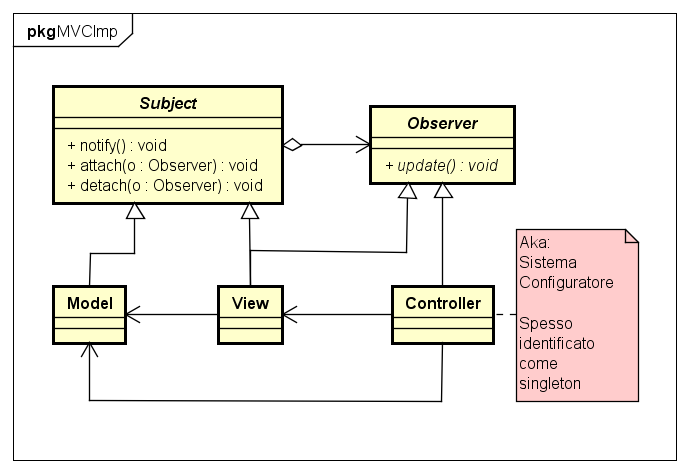
\includegraphics[width=\textwidth]{classDiagramPattern/MVCImp/MVC-Observer-Singleton}
					\caption{MVC - Observer - Singleton}
					\label{fig:MVC-Observer-Singleton}
				\end{figure}
	
	\begin{quote}
		\textit{"Il gioco deve disporre di un'interfaccia grafica basilare, che permetta all’utente di scegliere le proprie mosse."}
	\end{quote}
	
	Quando specificato che l'interfaccia è interattiva con l'utente usare l'\textbf{OBSERVER} con MVC, se non è solo l'utente a interagire, ma anche il sistema, utilizzare l'\textbf{OBSERVER} in entrambi i casi: \textbf{View-Controller} e \textbf{Model-View} (subject-observer)
	
	\begin{quote}
		\textit{"Il configuratore fornisce una UI interattiva, ma semplice all’utente."}
	\end{quote}
	Il \textbf{CONFIGURATORE} è un'altra figura che rappresenta il \textbf{Controller}, solitamente fornisce qualcosa.
	

\newpage
	\subsection{Polimorfismo}
	
	\begin{quote}
		\textit{"Ogni giocatore può essere guidato da un utente o dal computer."}
	\end{quote}
	
	Quando si specifica che una probabile tipo di oggetto può essere di diverse tipologie usare il POLIMORFISMO.
	
	\begin{quote}
		\textit{"Amazon ha prodotto molte versioni del sue reader, attualmente ne esistono due: kindle e kindle paperwhite. Entrambi usano il medesimo sistema operativo."}
	\end{quote}
	
	Attenzione, mentre qui sembrerebbe necessario il POLIMORFISMO la seconda frase dice di evitarlo poiché il SISTEMA è il medesimo, ciò significa che la differenza non è a livello di Business logic per cui il SISTEMA (il Controller) sarà unico.
	
	\textbf{Nota:} quando si hanno dubbi sull'uso di un'interfaccia e una classe astratta o classe, optare per la prima se si è sicuri che tale interfaccia non utilizzi altre classi, usare una classe concreta per tutti gli altri casi anche se fare una gerarchia con classi concrete è pura follia. Fare ciò per evitare la presenza di errori.
	
	\begin{quote}
		\textit{"Esistono due tipi di frame: quello di HD e quello in UHD"}
	\end{quote}
	In questo caso rispetto al \textbf{POLIMORFISMO} si preferisce utilizzare un \textbf{ENUM}.
	

\newpage
	\subsection{Abstract Factory Pattern}
	\begin{quote}
		\textit{"Amazon ha però voluto distinguere alcuni tratti delle UI di conseguenza pulsanti, slider e liste di articoli hanno un look-and-feel differente nei due e-reader."}
	\end{quote}
	
	Questo sta a significare che si ha una famiglia di prodotti diversi con tipologie diverse, è il caso di utilizzare un \textbf{ABSTRACT FACTORY} per ogni prodotto così da disaccoppiare i tratti grafici (item grafici) implementati dalla\textbf{ View}. Nel caso presentato le due tipologie di item sono quelle dei due tipi di Kindle.
	
	\begin{quote}
		\textit{"In particolare è richiesto loro di progettare una componente, ossia pulsanti. Questi possono essere di tre tipologie, ossi a pulsanti semplici, situati in una barra di navigazione o in una scheda (tab). L'aspetto di questi pulsanti deve essere omogeneo tra loro, ossia afferire alla stessa famiglia di oggetti"}
	\end{quote}
	
	Altro esempio in cui si necessita l'utilizzo di un \textbf{ABSTRACT FACTORY}, si riconosce per la presenza della parola 'famiglia' e 'tipologie' e la necessità di utilizzare \textbf{POLIMORFISMO} e disaccoppiamento delle componenti. Attenzione che per utilizzare una \textbf{ABSTRACT FACTORY} c'è la necessità di definire una \textbf{FACTORY} concreta, il testo la, o le se sono più di 1, suggerisce sempre.
	
	\begin{quote}
		\textit{"I modelli per cui la casa fornisce la configurazione online sono i propri modelli di punta, ossia il modello A ed il modello B."}
	\end{quote}
	
	Anche qui si ha una famiglia di prodotti: A e B, per ogni tipologia di accessorio si utilizza una gerarchia differenziata per il modello, in poche parole \textbf{ABSTRACT FACTORY}. 
	
	

\newpage	
	\subsection{Decorator Pattern}
	
	\begin{quote}
		\textit{"La configurazione riguarda gli aspetti più comuni dell'auto, ossia i cerchi (in lega e non) \dots"}
	\end{quote}
	
	Ogni qual volta si ha un particolare oggetto con una estensione bisogna pensare al \textbf{DECORATOR}.  Dalle soluzioni però non sempre viene utilizzato e talvolta viene utilizzato erroneamente. Il consiglio quindi resta di inserirlo solo se si ha certezza quasi assoluta che ci stia. Attenzione a non confonderlo con l'\textbf{ABSTRACT FACTORY} nel caso in cui ci siano famiglie di elementi e ci sia la necessità di rappresentarle per tipologie differenti, la loro costruzione avviene sempre tramite \textbf{ABSTRACT FACTORY} e mai si utilizza un \textbf{DECORATOR}.

	Si fa uso del \textbf{DECORATOR} soltanto quando nel testo si richiede di aggiungere funzionalità ad un oggetto.
	
	
	\subsection{Proxy Pattern}
	
	\begin{quote}
		\textit{"La sorgente del programma e la componente osservatore sono dislocate su macchine differenti, ma interagiscono fra loro come se condividessero lo stesso contesto di esecuzione"}
	\end{quote}
	Quando si parla di componenti su macchine differenti è il classico problema che risolve un \textbf{PROXY}.
	
	
	% ------------------------------
	
	

\newpage	
	\section{Diagrammi dei casi d'uso}
		
		\subsection{Identificare un caso d'uso}
		Molto spesso ogni caso d'uso proviene da una frase:
			
			\begin{quote}
				oggetto + predicato + complemento oggetto -> (esempio: "La registrazione avviene fornendo username e password")
			\end{quote}
			
			
		Ogni frase elementare (costituita dalla terzina) è un use case al 100\%. Nel caso dell'esempio abbiamo due casi d'uso che mappano in uno più generale: 'La registrazione' è il caso d'uso generale (oggetto), le frasi semplici, ossia i casi d'uso più atomici, sono:
		\begin{itemize}
			\item \textit{'La registrazione avvine fornendo username'};
			\item \textit{'La registrazione avviene fornendo password'}.
		\end{itemize}
				
		L'oggetto è in comune per cui è il caso d'uso generale delle due frasi semplici estrapolate dall'esempio. Il predicato si trasforma nell'azione di un ipotetico utente. Le due frasi quindi specializzeranno il caso d'uso generale in un nuovo diagramma.
		
		\subsubsection{Generalizzazione o specializzazione?}
		Si utilizza la \textbf{generalizzazione} nei casi in cui il caso d'uso principale è esteso e il caso d'uso eredita il suo comportamento specializzandolo. Notare che la \textbf{generalizzazione} tra casi d'uso è sempre la soluzione corretta nei casi in cui il testo descriva due comportamenti differenti per un unico caso d'uso utilizzando logicamente un OR (ad esempio quando si condivide qualcosa attraverso i vari social network o come nel caso della Ricerca spiegata in seguito).


\newpage
	\subsection{Probabili casi d'uso}
	
	
	\subsubsection{Registrazione} 
	Sempre un use case a parte specializzato con l'inserimento di USER o MAIL e PASSWORD con qualche <<extend>> di errore;
	
				\begin{figure} [h]
					\centering
					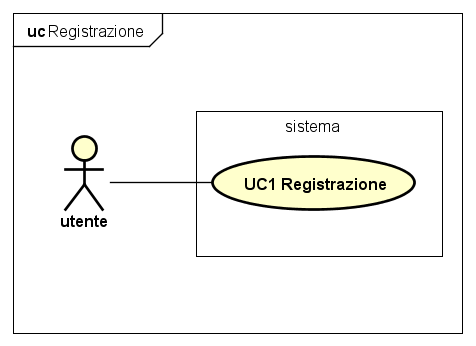
\includegraphics[scale=0.5]{UseCasePattern/Registrazione/Registrazione}
					\caption{Caso d'uso generale Registrazione}
					
				\end{figure}
				
				\begin{figure} [h]
					\centering
					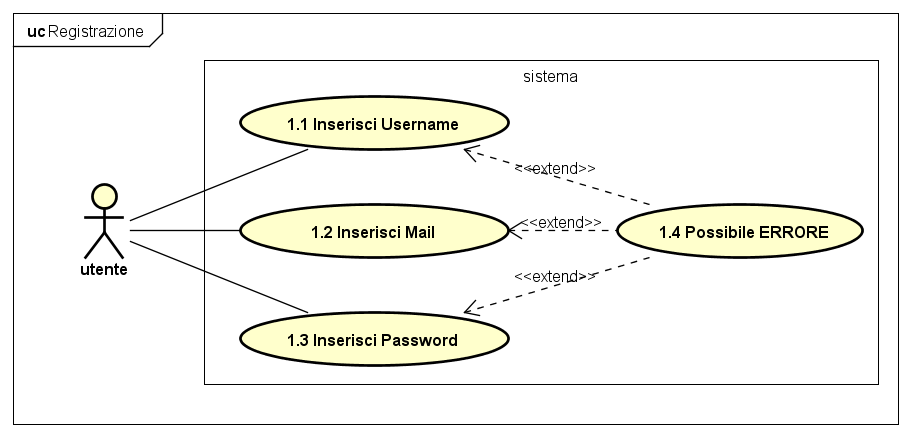
\includegraphics[scale=0.5]{UseCasePattern/Registrazione/RegistrazioneDettaglio}
					\caption{Caso d'uso in dettaglio Registrazione}
				\end{figure}
	
	\newpage
	\subsubsection{Utenti} 
	Spesso il caso è questo:
		\begin{enumerate}
			\item Utente non autenticato: ossia colui che può registrarsi, fare il Login e effettuare quelle operazioni definite spesso pubbliche.
			\item Utente autenticato: ossia colui che si è loggato e può effettuare più operazioni oltre a quelle pubbliche. Solitamente non è indicato quest'ultimo punto per cui non serve una gerarchia di utenti. Nel caso servisse vedere il diagramma dei casi d'uso:
		\end{enumerate}								
					
		\begin{figure} [h]
			\centering
			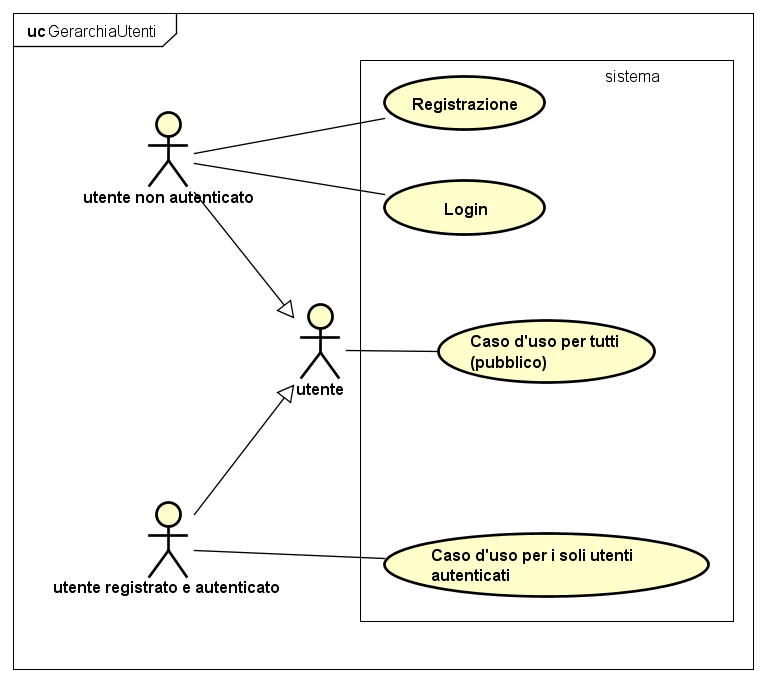
\includegraphics[scale=0.50]{UseCasePattern/GerarchiaUtenti/GerarchiaUtenti}
			\caption{Gerarchia utenti generica}
		\end{figure}
		
		\begin{figure}
			\centering
			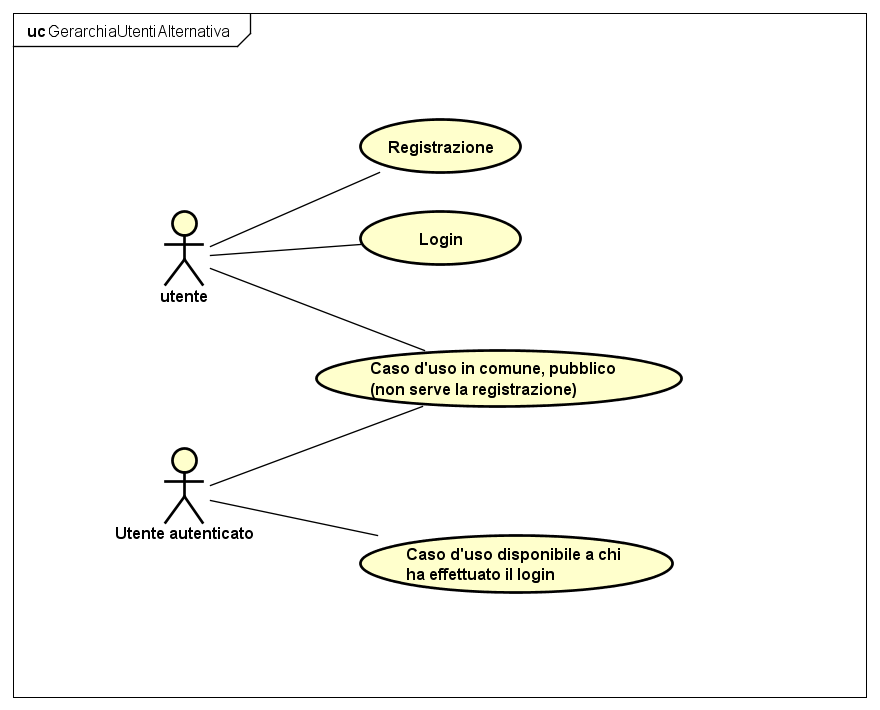
\includegraphics[scale=0.5]{UseCasePattern/GerarchiaUtentiAlternativa/GerarchiaUtentiAlternativa}
			\caption{Gerarchia utenti generica alternativa}
		\end{figure}
					
					
								
	\subsubsection{Altri utenti} 
	L'utilizzo di altri utenti avviene nel caso si definisca il chi manipola dei dati esternamente dal nostro sistema (solidamente altri sistemi come Google, Twitter, Banca, Facebook etc). In particolare nelle condivisioni spesso si ha il caso di utilizzare un ulteriore attore esterno al quale accade qualcosa (condividi su facebook -> uso di Server Facebook come attore esterno), talvolta questo caso è insieme ad una \textbf{generalizzazione}.
	Gli utenti esterni non devono essere mai utenti della nostra applicazione. Nel caso si riferisca ad altri utenti nel testo della consegna si consideri tali utenti gli stessi con cui si sta già lavorando. Ad esempio \textit{"viene inviata una notifica ad un destinatario il quale può visualizzarla"} il destinatario non è altro che l'utente che stiamo manipolando ossia anche colui che causa l'invio di una notifica. In questo caso infatti basterà aggiungere il caso d'uso \textit{Visualizza notifica} nei casi d'uso generali dell'utente della nostra applicazione, nient'altro.
					
	\newpage			
	\subsubsection{Ricerca}
	Spesso il caso si divide in una generalizzazione dell'UC generico 'Ricerca...' nelle tipologie di 'Ricerca' descritte. Seguire il diagramma:
	
		\begin{figure} [h]
			\centering
			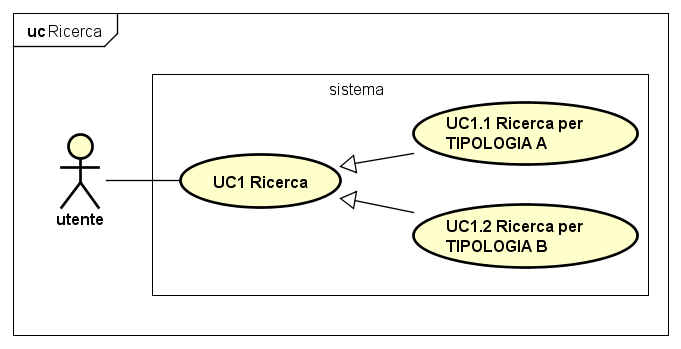
\includegraphics[scale=0.50]{UseCasePattern/Ricerca/Ricerca}
			\caption{Ricerca generica}
		\end{figure}
			
			
	\newpage	
	\subsubsection{Lista di item} 
	Spesso si trova che l'utente può visualizzare una lista, poco dopo sarà descritto cosa potrà visualizzare in dettaglio. In questi casi sempre:
		\begin{enumerate}
			\item Specificare il caso d'uso 'Visione lista item' con 'Visualizza desc items' o 'Visualizza titoli items' etc. come descritti. Ricordarsi di specificare le cose sempre al plurale in questo caso poiché si sta trattando un insieme di elementi.
			\item Inserire il caso d'uso generale: 'Visualizza dettagli item' e poi specificarlo con 'Visualizza dettaglio A', 'Visualizza dettaglio B' etc.
		\end{enumerate}
	
		\begin{figure} [h]
			\centering
			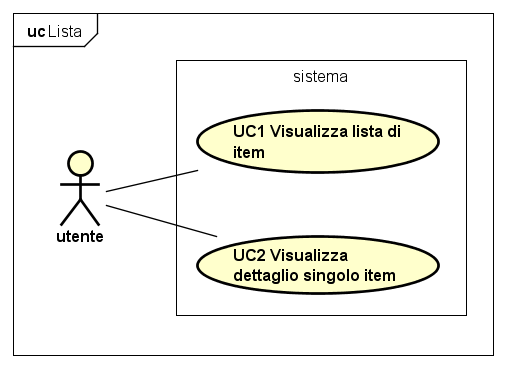
\includegraphics[scale=0.50]{UseCasePattern/Lista/Lista}
			\caption{Lista generica}
		\end{figure}
		
		\begin{figure} [h]
			\centering
			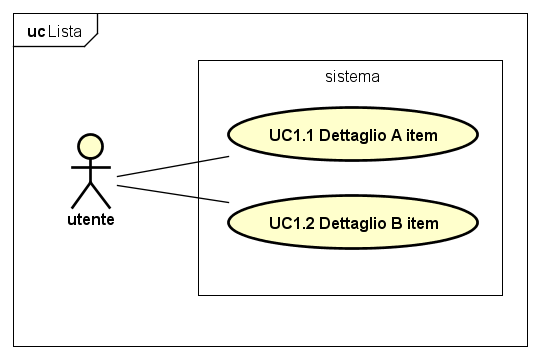
\includegraphics[scale=0.50]{UseCasePattern/Lista/ListaDettagli}
			\caption{Dettagli item visualizzabili nella visione d'insieme della lista generica}
		\end{figure}
		
		\begin{figure} [h]
			\centering
			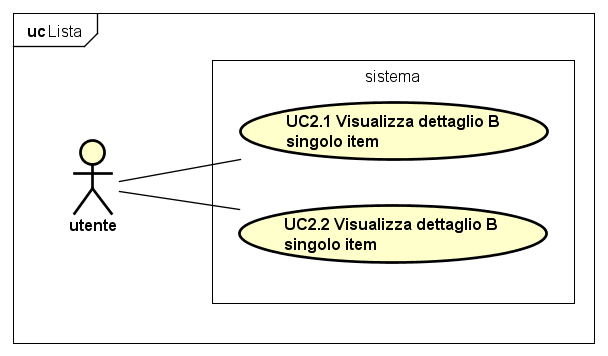
\includegraphics[scale=0.50]{UseCasePattern/Lista/ItemDettagli}
			\caption{Dettagli singolo item}
		\end{figure}
		
		
		\newpage
	\subsubsection{Condizioni}
	Quando nel testo si descrivono condizioni (ad es.: maggiore di N cose) si è in presenza di un <<extends>> obbligato. Nel caso d'uso che può generare in base al soddisfacimento della condizione dovrà essere appesa l'estensione del possibile avvenimento come mostrato nel diagramma:
	
		\begin{figure} [h]
			\centering
			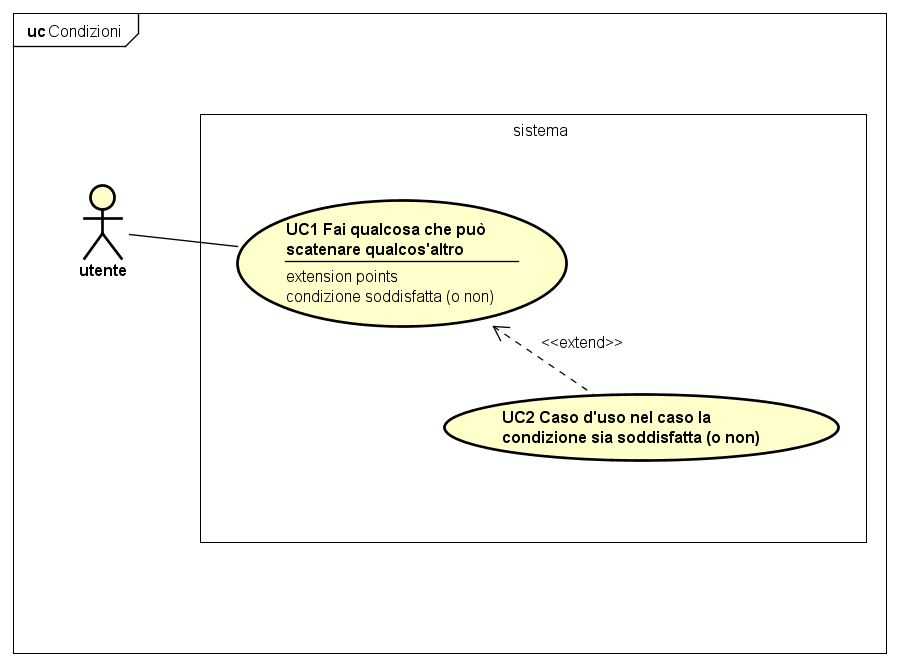
\includegraphics[scale=0.5]{UseCasePattern/Condizioni/Condizioni}
			\caption{Uso di notazione \textit{extends} e di una condizione}
		\end{figure}
			
	\subsubsection{Inclusioni} 
	L'uso di <<include>> si ha nei casi in cui il sistema a seguito di un caso d'uso fa qualcos'altro. Ad esempio un controllo sui dati inseriti. In generale l'inclusione si utilizza quando un caso d'uso dipende da un altro (relazione di inclusione). Dalle soluzioni riportate non viene mai usato, per cui nel minimo dubbio si \textbf{sconsiglia} sempre l'utilizzo di essa.


\end{document}